\chapter{Approaches}
\label{ch:approaches}

This chapter explains the process considered to answer the Research Questions. \\ \\

The Thesis work follows the Deduction research approach where the theory is established based on own ideas in addition to literature review findings. \\ \\

The prototypes are created based on the established theory and user study mentioned in Evaluation chapter \ref{ch:evaluationplan} is performed which follows Qualitative and Quantitative approaches in assimilating the results. It follows a well established Iterative process of UX Design \cite{UX} cycle as seen in the figure \ref{fig:ux-design}. \\ \\

Our approach leads an iterative process where initially prototypes with our novel ideas are evaluated by the target users. Next, the evaluation results lead to the requirements gathering phase. Then again, the prototypes are developed and so on the cycle repeats until the desired satisfaction of target users is achieved. \\ \\

In our Qualitative research methodology, the feedback of users is concerned as an example of emotional feeling on the usability of the designed prototype. Example: user behaviour, quotes etc. On the other hand, in our Quantitative research methodology, we analyse some metrics on the results gathered during the evaluation phase.  Example: time taken to perform the task, performance etc. \\ \\

For every Research Question, the user scenario is formulated and what usual Static Code Analysis tool does. Next, what can be done better considering other solution ideas from different Software Engineering domains in addition to our own ideas is analysed through the UX Design process. In this process, the metrics mentioned above which are Qualitative and Quantitative are observed.  \\ \\


Here is an example of how the implementation approach could get started. \\ \\

\textbf{Research Question}: How to display results from the same codebase from different analysis tools? \\ \\

\textbf{Solution ideas}: \\ \\
1. Display results separately for each tool \\
2. Combine the results and mark its respective icon in a column to indicate which tool identified the certain bug. \\ \\

With above-mentioned solution ideas, two different prototypes are designed using a wireframe tool called Balsamiq \cite{B}. Assume the name \textit{toolShort} mean a Static Analysis tool capable of giving results in short time and \text{toolLong} mean a Static Analysis tool gives results after long time. \\ \\

\textbf{Prototype 1}: \\ \\

The prototype for solution idea i.e., displaying the results separately is shown in following figure \ref{fig:toolSeperate}. \\ \\

\begin{figure}[hbt!]
	\centering
	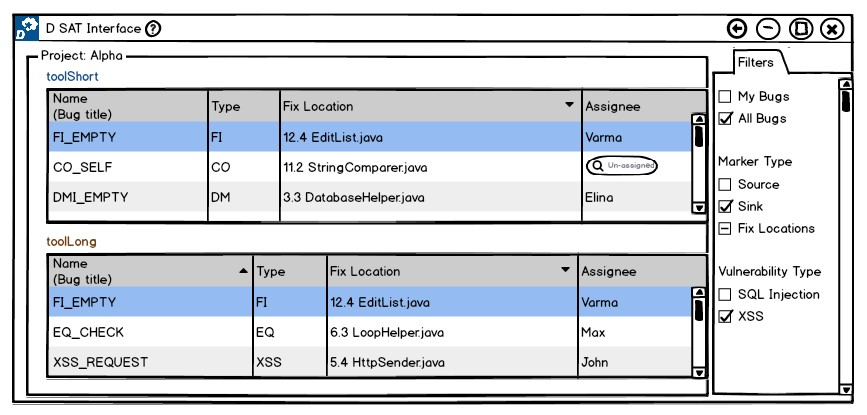
\includegraphics[width=\linewidth]{figures/d_seperate}
	\caption{An interface prototype with tools displaying results separately.}
	\label{fig:toolSeperate}
\end{figure}
\newpage

\textbf{Prototype 2}: \\ \\

The prototype for solution idea i.e., combining the results is shown in following figure \ref{fig:toolCombine}. \\ \\

\begin{figure}[hbt!]
	\centering
	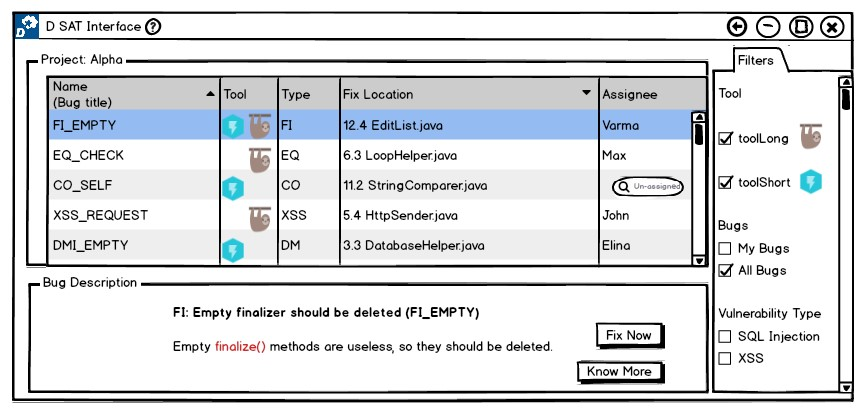
\includegraphics[width=\linewidth]{figures/d_combine}
	\caption{An interface prototype with tools displaying results combined.}
	\label{fig:toolCombine}
\end{figure}

\let\cleardoublepage\clearpage